% BSP for Bachelor in Game Programming
% english instead of norsk
% oneside for delivery, twoside for book style
\documentclass[BSP,english,oneside]{classes/gucthesis}

% For utf8 encoded .tex files
\usepackage[utf8]{inputenc}

% For colouring text
\usepackage[usenames,dvipsnames]{xcolor}

% For cross references in pdf
\usepackage[pdftex]{graphicx,hyperref}
\hypersetup{
	colorlinks=true,
	% linkcolor=Mahogany,
	linkcolor=MidnightBlue,
	citecolor=MidnightBlue,
	filecolor=MidnightBlue,
	urlcolor=MidnightBlue
	% linkcolor=blue,
	% citecolor=blue,
	% filecolor=blue,
	% %urlcolor=RoyalBlue
	% urlcolor=blue
}

% When linking to figures, link to their top, not the text underneat
%\usepackage[hypcap]{caption}	% throws warning..

% Put \capstart after \figure{}[] to get linking right
\usepackage{hypcap}

% To let figures float to side with text next to it
\usepackage{wrapfig}

% For math
\usepackage{amsmath}

% For appendix title
\usepackage{appendix}

% For footer on project frontpage
\usepackage{fancyhdr}

% For glossaries
\usepackage[nopostdot]{glossaries}
\usepackage{glossaries-babel}
\newglossaryentry{serialization}
{
	name=serialization,
	description={creates an internal representation of the visible data 
  				structure}
}

\newglossaryentry{ECMAScript}
{
	name=ECMAScript,
	description={Popularly known as Javascript, the most used scripting
				language throughout the web}
}

\newglossaryentry{Augmented Reality}
{
	name=Augmented Reality,
	description={A technology that enhance reality by combining digital and
				natural content, typically by combining camera, screen and
				processing power.}
}

\newglossaryentry{AR}
{
	name=AR,
	description={See \gls{Augmented Reality}}
}

\newglossaryentry{Vuforia}
{
	name=Vuforia,
	description={A free Augmented Reality software development kit that	offers
				vision-based image recognition for mobile platforms	and 
				Unity3D.}
}

\newglossaryentry{Inspector}
{
	name=Inspector,
	description={An area in the Unity Editor where you can manage editable
	properties of selected objects. In a script this can be public
	variables. In an object it can be position in space, scripts that are 
	attached, shaders that are used, etc.}
}

\newglossaryentry{Frame Marker}
{
	name=Frame Marker,
	description={A image recognized by the AR library as an object to be tracked and shown augments on.}
}

\newglossaryentry{Meta SpaceGlasses}
{
	name=Meta SpaceGlasses,
	description={Glasses that have screen capability on each eye. It features a camera and is therefore perfect for creating exiting experiences with \gls{Augmented Reality}}
}

\newglossaryentry{prefab}
{
	name=prefab,
	description={A premade object that can be added to the hiearchy in Unity, this object can have already added behavior as is the case with the camera used for our \gls{AR}.}
}

\makenoidxglossaries

% For including pdfs
\usepackage{pdfpages}

% For gantt chart
\usepackage{pgfgantt}

% Make chapters continue on same page
	% \makeatletter
	% \renewcommand\section{\thispagestyle{plain}%
	%                     \global\@topnum\z@
	%                     \@afterindentfalse
	%                     \secdef\@chapter\@schapter}
	% \makeatother


% Remove '%' in front of \renewcommand the parent command

% Create command for commenting
\newcommand{\comment}[1]{\textcolor{blue}{\emph{#1}}}
%\renewcommand{\comment}[1]{}

% Create command for todo things
\newcommand{\todo}[1]{{\par\noindent\textbf{\textsc{\color{Gray}todo:}}\color{Green}#1}}

% Norwegian Characters,  needs the {} or to be separate from the next letters
% \o{}   \aa{}   \ae{}   so at the end of a word you can use \o  \aa   \ae
% \O{}   \AA{}   \AE{}   you can also just leave a space and latex will remove it
%                        eg,  H\o gskolen i Gj\o vik

% \inlineHeader gives a header that does not show up in the table of content
\newcommand{\inlineHeader}[1]{\addvspace{1.5em}\noindent\makebox[\textwidth][l]{\large\bfseries #1}}


\begin{document}

\thesistitle{cogARC}
\thesisauthor{Per Kristian Warvik}
\thesisauthorA{Daniel Granerud}
\thesisauthorB{Jakob Sand Svarstad}
%\thesisauthorC{}
\thesissupervisor{Simon McCallum}
%\thesissupervisorA{} %second supervisor

\gmtkeywords{Bachelor, Thesis, Games, AR, cubes, IMT, cognitive, Augmented Reality}
\gmtdesc{Minigame environment with cubes in an augmented reality setting.}
\gmtnumber{18} % this is the number given to your project. May not be used  

\gmtoppdragsgiver{\GUC, Konstantinos Boletsis}
\gmtcontact{Konstantinos Boletsis, konstantinos.boletsis@hig.no, 12345678}




\thesisdate{\gucthesisdate}
\useyear{19.05.2014}

\gmtappnumber{} %number of appendixes
\gmtpagecount{} %currently auto calculated but might be wrong


\thesistitleNOR{cogARC}
\gmtkeywordsNOR{Bacheloroppgave, IMT, Spill, Utvidet Virkelighet, Kognisjon, Datasyn}
\gmtdescNOR{Denne oppgaven omhandler et milj\o{}  for \aa{} lage mini-spill som
kan brukes til kognitiv forskning. Teknologien som brukes er Augmented Reality.
Spillene l\o ses ved \aa{} flytte p\aa{} kuber med mark\o rer.}


% Create frontpages according to the school template
\makefrontpages

% Create project specific frontpage
\input{includes/cogarc_frontpage}

% Start counting pages after frontpage
\clearpage
\setcounter{page}{1}



% Preface (the * means do not give the chapter a number)
\chapter*{Preface}
	\label{chap:preface}
	Thanks goes to Costas B. for being a great employer and giving us good feedback
throughout the project. He has been availible and able to give answers when we
needed it.


\tableofcontents
\listoffigures

%%%%%%%%%%%%%%%%%%%%%%%%%%%%%%%%%%%%%%%%%%%%%%%%%%%%%%%%%%%%%%%%%%%%%%%%%%%%%%%
%%% PAGE COUNTING STARTS HERE %%%%%%%%%%%%%%%%%%%%%%%%%%%%%%%%%%%%%%%%%%%%%%%%%
%%%%%%%%%%%%%%%%%%%%%%%%%%%%%%%%%%%%%%%%%%%%%%%%%%%%%%%%%%%%%%%%%%%%%%%%%%%%%%%

% Start with content and count from 1.
\newpage
\pagenumbering{arabic}
% Put introduction here
\chapter{Introduction}
	
	%\section{Introduction}
		\setcounter{page}{1}	% Needed to get numbering right
		\label{sec:introduction}
		cogARC is a bachelor project under Gj\o vik University College. We have been
working with \gls{Augmented Reality} to create a tool for cognitive research.
The tool has form as a game with logging functionality that can be used by
researchers. cogARC can typically be used by patients that has suffered stroke
or people with declining cognitive functionality. Doctors, medical staff and/or
researchers can use logging information to get an overview over the cognitiv
situation for the patient and can be enabled to track improvements or
deterioration.

\cite{GenVirtual}

\chapter{Development Team}
The development team consisted of Jakob Sand Svarstad, Per Kristian Warvik and Daniel Granerud.
All of them were taking the bachelor game programming course at Gj\o vik University College for the last three tears from the autumn of 2011. One of the members had never seen a line of code before attending Gj\o vik University College while the two others had some experience with coding.

Two of the team members have worked together continuously troughout the  troughout the their time at Gj\o vik University College, but as a team we have only worked together on one project. We found out that we worked well together on that project and decided that we would work well together on a bigger project as well.

\chapter{Externals}

\section{Employer}

\section{Supervisor}
Our supervisor for this project has been Simon McCallum.

% \chapter{Project Description}

% \section{Reasons for creating this thing}

% \section{Implementation plan}
% %How we planned to implement this

% \section{Group Organization}
% %How we as a group organized ourself and the work

% \section{Report Organization}
% %How the report is organized, what each chapter is and short about structural layout.

% \section{Project Goals}
% %Our goals in this project, how far we want the project to go and how complete we hope it will be. What parts will be implemented and such



% What is the setting of the problem? This is, in other words, the background. In some cases, this may be implicit, and in some cases, merged with the motivation below.
% What exactly is the problem you are trying to solve? This is the problem statement.
% Why is the problem important to solve? This is the motivation. In some cases, it may be implicit in the background, or the problem statement itself.
% Is the problem still unsolved? The constitutes the statement of past/related work crisply.
% Why is the problem difficult to solve? This is the statement of challenges. In some cases, it may be implicit in the problem statement. In others, you may have to say explicitly as to why the problem is worthy of a BTech/MTech/PhD, or a semester project, as the case may be.
% How have you solved the problem? Here you state the essence of your approach. This is of course expanded upon later, but it must be stated explicitly here.
% What are the conditions under which your solution is applicable? This is a statement of assumptions.
% What are the main results? You have to present the main summary of the results here.
% What is the summary of your contributions? This in some cases may be implicit in the rest of the introduction. Sometimes it helps to state contributions explicitly.
% How is the rest of the report organized? Here you include a paragraph on the flow of ideas in the rest of the report. For any report beyond 4-5 pages, this is a must.

	\section{Description and goals}
		\label{sec:description_goals}
		\subsection{What is cogArc?}
cogARC is a small framework that uses Unity and the Vuforia library to let you make a selection of mini games where the user can move a set of frame markers in real life and see them interact on a screen that augments the game.

\subsection{Background}
This project is part of the PhD project done by Konstantinos (Costas) Boletsis. Our aim is that this project will help him in documenting a users cognitive changes by playing an assortment of mini games. In these games the player moves digitally recognizable items around in the real world and an augmented reality device will show the player the goals for the game. We have created software that offer games for the player and logging information for our employer.

\subsection{Why this task?}
We chose this task primarily because it gave us an opportunity to work with several technologies that we previously had little or no experience with.
It also gave us good experience in the rapidly growing field of \gls{Augmented Reality}. 
One major factor that triggered us was that we were supposed to work with the 
\gls{Meta SpaceGlasses}. Unfortunately we never got them, but that was a
calculated risk. Instead we used an Android powered tablet.

\subsection{Target demographic}
The target demographic for the finished product is healthy people that are at high risk of cognitive decline. This can include, but is not limited to, seniors with mild cognitive impair and people that has suffered stroke.
Our employers hope is that by using this product he can measure the cognitive performance and possibly keep track of cognitive changes over time (if there is any).

\subsection{Goals}
The task we initially got was to create some mini-games using \gls{Augmented Reality}. Many of these games had many similar features, so we decided to have a different approach to the task. The goal we sat before us was to create a program, an environment, for making these games. We wanted the environment to enable our employer to manipulate the games we had created for him. It should also be able to use the features we had implemented to create new games. This should be done without changing a lot of source code and hopefully save valuable time.


\begin{description}
	\item[To be more precise, this is our goals:]\ 
	\begin{itemize}
		\item Functional \gls{AR} games.
		\item A manipulative environment.
		\item Implemented features available for creating similar games. 
		\item Interface through Unity's \gls{Inspector}.
	\end{itemize}
\end{description}


\subsection{Augmented Reality}
"Augmented reality (AR) is a live direct or indirect view of a physical, real-world environment whose elements are augmented (or supplemented) by computer-generated sensory input such as sound, video, graphics or GPS data. It is related to a more general concept called mediated reality, in which a view of reality is modified (possibly even diminished rather than augmented) by a computer. As a result, the technology functions by enhancing one’s current perception of reality. By contrast, virtual reality replaces the real world with a simulated one. Augmentation is conventionally in real-time and in semantic context with environmental elements, such as sports scores on TV during a match. With the help of advanced AR technology (e.g. adding computer vision and object recognition) the information about the surrounding real world of the user becomes interactive and digitally manipulable. Artificial information about the environment and its objects can be overlaid on the real world."\cite{WikiAugmentedReality}



\chapter{Organization}

\subsection{Implementation plan}
To implement this project we worked Monday to Thursday.
Friday was left to do other courses as each member of the class had signed up to at least one other class.
Exceptions to working on Monday to Thursday was made when it was needed.

On the scheduled days we sat together to coordinate what needed to be done and how progress was going so we could quickly re-plan when needed.
Most of the time we worked one by one although we sat together.
This let each member work at home if they wanted to go home to work or do the work at another time if they so wanted to.
If something needed multiple heads on the job this was then easily done as we was in the same room.

Delegation of work was done by the group as a whole where tasks was given to either the person most fitted to doing it based on previously shown skills, or if some one really wanted to do a task it would be given to that person. We did it like this as we saw this to be the fairest way.

At the end of each work week (Thursday) we held a short weekly meeting to asses what had been done by each member and what had been achived by the team.
We also wrote down what we planned to do the next week.
This way it was easy to track what had been done and what was to be done.
\todo{Is this enough?}

\subsection{Group Organization}
	\todo{Fill this one out better? Yes, a lot better would be nice.}
As a group we tried to organize ourselves so the workload would be as equal as possible. 
We had a group leader in name only as there was never a need to resolve a conflict within the group.
Although we tried to keep the workload equal it was split a bit between the three developers due to practicalities. 
For instance the work of doing the internal game logic was left to almost solely one developer as this required a lot of work with a few algorithms and little else.
We therefore saw it fitting to have one member of our group almost solely responsible to make it work whilst the two other developers did the other parts.
Although one developer was responsible for one thing we made sure that everyone on the team knew as much about every part as possible, in case one became sick or otherwise indisposed we would not be left with a big piece of work the others then would know nothing about.


\subsection{Report Organization}

\todo{How the report is divided and reasoning behind the dividing.}
\todo{How the report is organized, what each chapter is and short about structural layout.}

Our report is structured into 6 parts where each part contains chapters that are related to the encompassing part.

\begin{enumerate}
	\item Introduction.
	\item Design process.
	\item Development process.
	\item Product.
	\item Summary.
	\item Appendices.
\end{enumerate}

Introduction will introduce you to the project and its developers.


Design process will tell you how we designed and approached the project around our given requirements.


Development process will describe the theoretical part of the project as well show how we worked and what we did and with which tools.


Product will show you what we ended up with at the end of our development.


Summary will round up the project and thesis with a conclusion and afterword.


Appendices is at the end and will contain a bibliography, glossary, how we managed time and other neat tidbits.


\todo{Rewrite appendices at the end. Make this pretty.}

	\section{History and Background}
		\label{sec:history_and_background}
		\subsubsection{Augmented Reality}

\gls{Augmented Reality} is a quite new discipline in computer science. It uses
a real-world environment and augments its perspective with adding digital
content. One of the biggest contributors in the field is Steve Mann, who has been
working with wearable computing and augmented reality systems since the 1980's.

The \gls{AR} term itself was coined at Boeing\cite{boeingAR} in 1990 where the
technology was
proposed to replace a lot of large plywood boards with schematics for planes.
They proposed a kind of eyewear that could project the schematics on reusable
boards and with this make reconfiguring a whole lot easier during the
manufacturing process.

Even though most of the AR technology of today happens through screens (like
mobile phones and Google glasses / Meta SpaceGlasses\cite{MetaSpaceGlasses}),
the id\'{e}a of projection is still living. castAR is an example of this 
technology where digital content is cast on a reflective material.
The technology has been around for some decades and is being present in several
forms, but the technology has needed a long time to mature. It is only recently
that algorithms and hardware has started to be good enough for everyday people
to take interest, and because of this we will still consider it as a quite new 
discipline in computer science.

\subsubsection{Serious Games}

\todo{Write some background related to Serious Games here..}\\

The background for the project is that our employer Costas Boletsis is doing
a PhD and wanted a set of games that tests the players cognitive condition
by completing defined tasks. To do this he wanted to use a device that
implements augmented reality on a set of physical cubes that the user can
interact with.

\todo{Merge the following text with \nameref{subsec:why_this_task}}\\
When we decided we wanted to go for the task, we were expecting to use the
Meta SpaceGlasses. They were expected to be released in December 2013, but
unfortunately the release of these has been pushed forward to July
2014\cite{MetaSpaceGlasses}.
\todo{The following text is more design and implementation. Should go further
down in the report.}\\
Because of this we have been developing for the Android platform. During the
development process we have tested on our own phones, but towards the end
of development, as well as during testing, we have also tested on a tablet.

\todo{Maybe merge this with the first paragraph in \nameref{subsec:goals}}\\
We got a set of game specifications that our employer wanted us to implement.
Many of the games had similar features, so we decided to do the project a
little more useful.
Instead of making several independent games, we decided to create a kind of 
platform or environment. In this piece of software we have tried to make it
easy to create and modify small games with a certain set of features. Our
hope is that our employer and others can use it as a tool to perform research
and medical analysis. The environment will contain predefined objects that
can be manipulated and put together to achieve different goals for measuring
a number of cognitive functions.

\subsubsection{Mild Cognitive Impair}

\todo{Find something to write here.. medical, abstract, something...}

	\section{Related work}
		\label{sec:related_work}
		\gls{AR} is a technology that is starting to get popular. Because of this there
are not that many contributions to the field that is too similar to our project.
At the University of S\~{a}n Paulo, some academics have created a musical AR game
that has noticeable similarities with our work, they have called it GenVirtual
\cite{GenVirtual}. 

There exists AR games both for entertainment and for more purposeful
measures\cite{tan2010augmented}. In 2000, ARQuake stood out as the first fully
working outdoor AR game. It needed a lot of equipment attached to the body, so
it was never commercialized. Anyway, it generated a substantial interest in the
AR community. From 2005 and onwards more AR games have appeared. As
equipment have become cheaper, lighter and less space consuming, it has opened a whole new world of possibilities. 
Smartphones and tablets have brought forth
small devices with increasing processing power. With freely available libraries
as \gls{Vuforia}, many new applications are expected.



\chapter{Design process}
	\label{chap:design_process}

	\section{Approach}
		\label{sec:approach}
		Seeing that Konstantinos Boletsis had created a design document for us to follow made the designing of the games easier.


Having the mini-games clearly defined ment that we could focus on other parts in the beginning of the project instead of having to design the games ourselves.
This let us focus solely on the interaction of the user and the program we made during the early stages of the project.

It also let us test the technologies a lot more without having to design around the limitations of the frameworks.


We approached the design of this a lot differently than we have approached problems in the past.
Being used to having interactions purely in the digital space let us design in a familiar environment where we could control all variables and interactions.

This is not something we could do in this project. 
We used a more emergent design process of trial and error to find out what worked and what did not work with using physical cubes along with a screen and camera.
For instance testing lighting conditions to find out when the frame markers was most easily found by the camera \& Vuforia (they work best in a well lit area with few sharp lights that gives reflections on the markers).

We also discovered many other interesting things while testing, for instance that if the virtual cubes are a bit larger than the cubes themselves it looks more believable than if it just as big,
 this might be due to the nature of augmented reality, or it is a quirk of Vuforia, but when a frame marker becomes partly occluded or untraceable but still visible enough that Vuforia recognizes it something peculiar happens.
Sometimes it looks like the viritual box is stuck even if the frame marker is moved or it can get a weird transformation, often making it appear a lot closer than it should be and more often than not also being at a odd angle.


Early on we found out that Vuforia supports having viritual buttons on image targets (unlike frame targets Vuforia can only track five image targets at a time) which projects an augmented button on the screen that the user can press as if it was a real physical button.

This would be a great addition to our project we tought and looked into adding viritual buttons.
Sadly we found that when using frame markers, Vuforia does not support virtual buttons. That ment that if we wanted to have viritual buttons we would have to either stop using frame markers or make a second set of cubes with image targets.

Using image targets comes with the downside that a maximum of five images can be tracked at a time. This is because of increased complexity when analyzing the camera input. The mini-games we are implementing require the ability to track up to ten targets at a time, so the id\'ea of using image targets had to be discarded.

Having another set of objects to track did not appear to be the best of ideas. 
Already having ten cubes to track is already quite a lot and having another set of trackable objects would have led to more fustration than easy of use for the user.
Ten cubes takes up a lot more physical space than one would originaly anticipate as they will end up being spread out to make it easier for the player.

\todo{More?}


	\section{Requirements}
		\label{sec:requirements}
		All requirements for this project was created based on a design document given to us by our employer.
As we were not given any concrete requirements outside of the design of the individual minigames we
were left to create them based on this.


\subsection{Operational requirements}
Based on the design document we were able to create a small set of goals that had to be reached for this project
to be considered complete and operational by us.
Based on the design document we created the goals of creating a set of minigames that:
%The goals of this project is to create a set of mini-games that:
\begin{itemize}
	\item Tests the players' cognitivity and to slow down their cognitive decline.
	\item Keeps track of the players' cognitive performance.
	\item Track and document the cognitive changes.
	\item Uses AR to provide a new experience.
\end{itemize}

\subsection{Functional requirements}
When considering functional requirements we found that there were some requirements that would have to be there to make the program do what the design document specified. 
The markers on the cubes would have to be seen. 
In our case we have used the library \gls{Vuforia} to handle all input from the camera.
This means that we had no influence on the direct observation on the cubes. 
Vuforia would analyze images from the camera and give us positions of the different trackers when they were observed. 
In our situation, the chance we had to influence here lies in how we handle the input we get. 
We have written more about this opportunity in chapter \ref{sec:AR_library_integration} \nameref{sec:AR_library_integration}.

\paragraph{Logging}
Our employer originally wanted us to log the hand movements of the user when the user is playing the game. 
With the META SpaceGlasses this is supposedly possible, but as of the writing of this report the SDK for the SpaceGlasses have yet to ship. 
In the beginning of the project we looked into doing this with the technology we were going to use for the project, Unity and Vuforia. 
We looked into this, but found that neither Unity or Vuforia support any kind of tracking of hands. 
We brought this issue to our employer and after telling him of our findings we were told that we could then drop logging of the players hand movements altogether. 
He said he also wanted logging of certain other events, but we could save this for last and do it if we had time to implement it.

%\subsection{Usability requirements}
%\todo{write}


	\section{User experience goals}
		\label{sec:user_experience_goals}
		As mentioned earlier, AR is a quite new technology which combines the physical 
world with the digital world. Since the technology is quite new, the experience
this gives is also new to many. We want the players to feel exited about using
this new technology. We also want the players to be cognitively stimulated and
feel challenged. At the same time we hope that it will be fun and entertaining
to play.


	\section{Usability goals}
		\label{sec:usability_goals}
		In this project we have been focusing on three usability goals\cite{rogers2011interaction}.

The first is utility. We want our game to be as easy to use as possible. The
games require the users to put cubes next to each other and solve a set of
different tasks this way. A strength with the software is that by using such
a simple action one can solve several different tasks.

The second usability goal is learnability. The tasks should be easy to
understand and easy to learn. The challenging factor should lie in the tasks
to be solved, not to understand the concepts. We have tried to solve this
with explanatory text. Since the games are quite simple in their nature we
hope this is enough. If we had better time we could have supplemented with
small animations.

The third usability goal we have focused on is memorability. When coming back
to cogARC, it should be easy to start up again without any need to relearn how
to use it. This is achieved by having a quite simple and repeatative interface.
Instructions are also small and repeated before each game, so there would be
little or no need to relearn anything.

	\section{Game descriptions}
		\label{sec:game_descriptions}
		\input{includes/cogARC_game_descriptions}


\chapter{Development process}
	\label{chap:development_process}

	\section{Theory}
		\label{sec:theory}
		\subsection{Gyroscope and directional vectors}

\begin{wrapfigure}{r}{0.4\textwidth}
        \capstart
        \vspace{-20pt}
        \centering
        \includegraphics[width=0.38\textwidth]{images/GyroObjectModel.png}
        \vspace{-20pt}
        \caption[Model of the game-object used to get the direction up]{Not the one we used in the application, but it illustrates the principle better without the extra functions. This object is fixed in the real world when the user rotates the device, so that the up-vector points up in the real world.} 
        \label{fig:Gyro_model} 
        \vspace{-10pt}
\end{wrapfigure}

Since one of the games required the player to build towers with the cubes and the project is about augmented reality, we thought it was a good idea to use the gyroscope rather than relying on the player to hold the phone the right way up. We also thought of using the gyroscope to separate four sides of interaction in the horizontal plane, but that is a compass and we couldn't expect the user to be facing north when playing the game. We could expect up to be up, but not west to be left, so for this we had to go with the Unity-world-coordinates with the camera as center. The problem was to know how to use the gyroscope.\\

\begin{wrapfigure}{l}{0.4\textwidth}
        \capstart
        \vspace{-20pt}
        \centering
        \includegraphics[width=0.38\textwidth]{images/CollisionDirectionObject.png}
        \vspace{-20pt}
        \caption[Model of the collision direction vector]{The vector shows the direction from the cube in focus to the colliding cube.} 
        \label{fig:Collision_Direction_model} 
        \vspace{-10pt}
\end{wrapfigure}

From a standard Unity function we got the rotation of the real world from the gyroscope. The optimal thing to do would be to rotate the Unity-world to be the same as this rotation. This however was not possible and the markers use global position so we couldn't make a virtual world object in Unity to rotate. We could have added the rotation to the cubes transforms, but we only needed to know the direction of collisions. \\
To solve this we made an object that get its rotation directly from the gyroscope. To this object we added a child object that has a local position one unit above the parent. Subtracting the global position of the parent from the childs global position gives us a unit vector for the direction up in the real world. This could have been done more effeciently without the objects, but it was important to have visual indications of directions for development and testing.\\

\begin{wrapfigure}{r}{0.4\textwidth}
        \capstart
        \centering
        \vspace{-10pt}
        \includegraphics[width=0.38\textwidth]{images/CollisionDirectionAngleModel.png}
        \vspace{-10pt}
        \caption[Model for finding the angle between the vectors]{The angle between the up-vector in the gyroscope-object and the collision-direction-vector from the cubes.}
        \vspace{-10pt}
        \label{fig:Vector_Angle_model}
\end{wrapfigure}

Then on collision we can take the direction-vector between the colliding cubes. 
\[
(cubeB.position - cubeA.position)
\]

% This is the figure containing math. I put in some LaTeX math instead...
% \begin{wrapfigure}{l}{0.4\textwidth}
%         \capstart
%         \centering
%         \vspace{-20pt}
%         \includegraphics[width=0.38\textwidth]{images/AngleFormula.png}
%         \vspace{-20pt}
%         \caption[Description]{A = collision-direction-vector, B = Up-vector, |x| = length of x, cos = cosine, acos = arc-cosine.}
%         \vspace{-10pt}
%         \label{fig:Angle_Formula}
% \end{wrapfigure}

\subsubsection{Degree vertical}
By normalizing the vectors you can use the scalar product or dot product between the two vectors to find the vertical angle between the cubes. However Unity actually has a function for finding the angles between vectors, so most of our difficulty lay in testing that everything worked the way we thought and rotations were not inverted, incorrectly rotated or too unstable to use.


\subsubsection{Calculate the angle}
\newcommand{\norm}[1]{\lvert #1 \rvert}

For calculating the angle we need the following prerequisites.
\[
A = \text{Collision direction vector}
\]
\[
B = \text{Up vector}
\]
\[
\norm{x} = \text{length of x}
\]

\paragraph{}
With this in place we can get the answer with a little bit of math:

\[
A \cdot B = \norm{A} \cdot \norm{B} \cdot \cos(angle)
\]
\[
A \cdot B = 1 \cdot 1 \cdot \cos(angle)
\]
\[
A \cdot B = \cos(angle)
\]
\[
\arccos(A \cdot B) = angle
\]


\paragraph{}
 The angle varies between 0-180 degrees. We have specified that less than 60 degrees means one is below the other. More than 120 degrees means one is above the other. If the angle varies between 60 and 120 degrees, cogARC will see it as a horizontal collision.

	\section{Tools}
		\label{sec:tools}

		\subsection{Unity}
			\label{subsec:unity}
			\todo{Why...?}
\todo{Generally how it works. Generally how it does not work. Generally how it make people cry.}
Unity Unity Unity, what is it and why do we hate it.

Unity is a game engine and development enviroment.
It features a intergrated work enviroment with good tools that promotes rapid workflows to create the games you wish to create without worrying about the underlying structure.
With its multiplatform deployment tools and intergrated asset store it has become very popular for games.
Supporting both 2D, 3D and animating makes so that you dont need other programs to create what you wish to create.

Getting into Unity for the first time is greatly aided by the many video tutorials that Unity has created, showing how to use the interface, basics of scripting and programming, how to add sound and much more.



		\subsection{Vuforia}
			\label{subsec:vuforia}
			\todo{Vuforia: Why...?}
\todo{Vuforia: Generally how it works. Generally how it does not work. Generally how it make people cry.}

		\subsection{MonoDevelop}
			\label{subsec:monodevelop}
			MonoDevelop is the integrated development environment (IDE) that comes with Unity. It supports writing in C\#, Unity JavaScript and Boo.
MonoDevelop is developed by Xamarin \cite{xamarinRef} as an open source integrated development environment for Windows, Linux and OS X.
Its primary focus is on C\# and other .NET languages.


MonoDevelop offers debugging features such as breakpoint, stepping trough code one line at a time, tracking of variables, call stack of functions and more.
It also have features to help with programming such as code completion and solution overview. Alongside all this it also supports add-in's for adding support for other languages.


\begin{wrapfigure}{l}{0.3\textwidth}
	\capstart
	\centering
	\vspace{-10pt}
	\includegraphics[width=0.28\textwidth]{images/MonoDevelopLogo.png}
	\vspace{-20pt}
	\caption[MonoDevelop IDE Logo]{{M}ono{D}evelop {IDE}}
	\label{fig:monodevelop}
	\vspace{-10px}
\end{wrapfigure}

For us MonoDevelop gave mixed results. 
I have no doubt that it is a good IDE for working with C\# or a .NET language, but the UnityScript integration is poorly done.
The auto complete functions was flimsy at the best of times, most of the time it never activated and when it did it did not give the correct results. 
There has also been times when trying to get a public variable have resulted in a error because the variable has yet to be defined while it is available two lines above with no change in the scope.
We believe these problems are more due to Unitys implementation of JavaScript and not a error on MonoDevelops part, so if one are to use MonoDevelop we would recomend to shy away from Unitys JavaScript and use C\# instead.
Ending with on a positive note it had the best "Watch" feature we have come accros, it made tracking of several variables at a time really simple even if that variable was part of another script or class.	

\todo{Does this need more?}

		\subsection{Third party libraries}
			\label{subsec:third_party_libraries}
			\paragraph{PlayerPrefsX}
PlayerPrefsX (also known as ArrayPrefs 2)\cite{PlayerPrefsX} is a library created by the Unity community to enhance the built in Player Preference class of Unity.

PlayerPrefsX expands Unitys' way of storing player preferences or other data that the programmer want to persist between sessions.
Unity without PlayerPrefsX supports saving and getting float values, int values and strings. Altough this is all that is needed in most cases, it is sometimes practical to be able to store a bit more complex data.

PlayerPrefsX is able to store vectors, quaternions, arrays and more. 
We used this library to store the list of high scores for each game. 
By using PlayerPrefsX IntArray storing it was very easy to store a array of ten high scores for each game instead of having to either make a complex string to store it or fining another way of storing the scores.

\paragraph{Boomlagoon.JSON}
\todo{PK: write about JSONObject}

			
		\subsection{GIT}
			\label{subsec:git}
			We have been using GIT for version control in this project. This is a version
control system we had some prior experience with, so we wanted to try it for 
this project as well. 

GIT works best with plain text files. With Unity there is quite many binary
files as well. At first we were not entirely sure how much of the files that
were binary and if GIT could work for us. After some googling we found that 
this was possible. On Unity's webpage they instruct on how to use the version
control system called Subversion \cite{SubversionControl}. Together with some
help from Stackoverflow.com\cite{gitVersionControl} we figured out how to set 
up the project with GIT.

Unity produces .meta-files for each file in the project. We do not know 
entirely how these works, so we met some problems that we suspected had its
origin in these files. Because of this we have tried both to have them in
the GIT repository and not. The solution to that specific problem was not
clear when we got it working, so we do not know whether the metafiles were
problematic or not. The post at Stackoverflow explained that the .meta-files 
could be set to hidden. This implies that the files should not be part
of the GIT repository. Anyway, now they are because it seemed to help with the
problem we had, and it has not given any other problems later.


\begin{wrapfigure}{l}{0.3\textwidth}
	\capstart
	\centering
	\vspace{-10pt}
	\includegraphics[width=0.28\textwidth]{images/git}
	\vspace{-5pt}
	\caption[GIT logo]{GIT}
	\label{fig:git}
	\vspace{-10pt}
\end{wrapfigure}

Many of the pure binary files has not been necessary to upload. Those that
has, like images, has often been of a type that didn't need to be updated
often. This means that most of the content in the repository could be plain
text and therefore we have been able to use GIT without further hassle.

\begin{wrapfigure}{r}{0.3\textwidth}
	\capstart
	\centering
	\vspace{-10pt}
	\includegraphics[width=0.28\textwidth]{images/github}
	\vspace{-5pt}
	\caption[{G}it{H}ub logo]{{G}it{H}ub}
	\label{fig:github}
	\vspace{-10pt}
\end{wrapfigure}

We have used GitHub \cite{GitHub} as our online repository server. By using
this service we could easily share the work we have done. That we could use
an external server like this has been important for us when choosing version
control tool. Especially in one occasion this proved to be very smart. One of
us encountered a bug in Unity that were quite severe. The Unity3D program
crashed, and by some unknown reason, it deleted a lot of files. The files that
were removed were all of the project files + some other files in the parent
directory. Many totally unrelated files were deleted and 4 days work that was
not committed to the server were lost. But fortunately enough, he could
download the latest version from GitHub and use the last days lessons to write
the lost changes a whole lot faster.

When we have been using GIT we have used the commandline tool and also the GUI
program for GIT called Sourcetree \cite{SourceTree}.

The workflow we have been using has been very simplistic. We are aware that
there are good workflows that we could have used, but we have chosen to only
have a master branch that everyone pushes to. During the project we were told
about a way that worked for another group were they used pull requests and in
this way added an extra layer of security of code integrity. We tried this out
for a short time, but since none of us had experience with this way of working,
we discarded it after a relatively short time. We were working quite close with
many small and rapid changes that we shared with everyone. If another group
member should accept this every time, we think that a lot of unnecessary time
could have been wasted on this. The model is not bad, but we have come to the
conclusion that it didn't fit our way of working very well. If we had started 
to do it from the beginning, we could maybe have done it, but the effort may
still have not been worth it. Anyhow, we are glad to learn about other ways of
working that can be useful later.

		\subsection{LaTeX (\LaTeX{})}
			\label{subsec:latex}
			We have chosen \LaTeX as the tool for writing our report. In the preplan we
made the document with Google docs \cite{GoogleDrive}. This worked ok, since
we all could work with the document at the same time. The functionality in that
editor is quite ok, but somewhat limited and hard for big projects. One is
also dependant on a stable Internet connection. None of the group members had
used \LaTeX notably before. Therefore we used some time on deciding whether we
should use it or not.


	\section{Schedule}
		\label{sec:schedule}
		We planned the development project and ended up with the gantt diagram shown in Figure \ref{fig:preplan_gantt}:

\begin{figure}[h]
	\capstart
	\centering
	\includegraphics[height=\textwidth, angle=270]{preplan_gantt_diagram}
	\caption[Preplan Gantt diagram]{Our initial gantt diagram for the project.}	\label{fig:preplan_gantt}
\end{figure}


Afterwards we see that the process has been like this:

\todo{Insert gantt diagram of our dev-process here.}

\section{Planning vs reality}%Or how we worked compared to the plan
Our development cycle deviated a lot from the original plan due to a multitude of factors.
For instance we could have allocated less time to the "Create application enciromnet and menu UI" and "Recognice cubes" which each were allocated 7 days in the plan, but had we known more about Unity or the Vuforia plug-in in Unity then we would have known that Unity have methods and functions for creating in-game UI and to make the Vuforia plug-in working were just adding a \gls{prefab} for the camera.
We spent the time allocated to those time slots to creating the framework instead and this additional time shifted a lot of the sub-sequential work a week ahead of time.
Task number 10 (Real world orientation (for besides and upon)) was moved to the beginning of the project by developer Jakob and was done as part of him learning Unity.

The most drastic change in the time schedule is in item 11-15.
After learning some of the inner workings of Unity and how to properly set up a game in Unity it became rapidly apparent that we had taken a somewhat naive approach on it. This was due to our lack of knowledge of how much a game engine can do for us.
Using Unity we had a almost complete mini-game enviroment from the beginning. As such we only had to program what interaction we wanted to happen when cubes collided.
Our time and efforts were then spent on making the interaction between cubes and the player to what we wanted instead of having to focus on making the basics of a game world working.


%	\section{Process}
%		\label{sec:process}
%		%Write aboot the development process
%Fuck yes

	\clearpage
	\section{UnityScript}
		\label{sec:UnityScript}
		In Unity a user can use several different languages to script their games. Boo, C\#, JavaScript and Shader (used for writing shaders).
While Boo and C\#  use the standard implementation and is easily referenced the JavaScript used in Unity is not.\cite{WikiScriptVSScript}

Unitys JavaScript is quite different in many ways from the more standardly used JavaScript that is based on ECMAScript\cite{ECMAscipt} which is a standardized scripting
language standardized by Ecma International.

Some of the major and notable differences between Unitys JavaScript (henceforth named UnityScript) and ECMASCripts JavaScript (henceforth referred to as JavaScript):

\begin{itemize}
	\item Classes.
	\item Different privacy.
	\item Not JavaScript library compatible.
\end{itemize}

\subsection {Classes}
JavaScript have no concept of classes as it is a prototypical language, meaning it will have the properties that is assigned to it, but is not bound to them.
Properties can be added or deleted at will in runtime, this is true for both members of the object and functions. 
UnityScript is much more object oriented with strongly typed and defined classes that cannot be changed in runtime (the exception to this rule is reflection).
This makes it difficult to work with UnityScript if you have little experience using it, or have yet to find out that the difference between JavaScriptand UnityScript.
UnityScript have also removed the prototypical properties of JavaScript by implementing it as a class based language. 
Meaning objects can not get additional functionality or be completely redefined at runtime. 
In UnityScript each .js file is implemented as a class by default. 
So when a developer creates a new .js file the Unity compiler and serialization system will add a class definition around the data within the file by default, so to call a function within a .js file you write "filename".function.
This however is not documented and gave us problems in the starting phase when we were learning UnityScript as there was no obvious way to get data or functions from other files.

\subsection {Different privacy}
UnityScript, being structured like other object oriented languages have the usual levels of privacy of members within a class being marked as either Private, Protected or Public. 
JavaScript have per function privacy. 
Meaning a variable declared in a function is available in the entire function but not outside of the function.
But sometimes the compiler gets this confused or ModoDevelop get this confused as we have had problems with a variable being accessible in one part of the function but not in other parts.
This has been the case with member variables of the script and variables in the function not being available, this led to having some times having to create temporary variables to store the original variable to be able to use it in the fucntion.
%
%\subsection {var as a keyword is required}
%If you do not use the keyword var in JavaScript the variable becomes a global variable as the var keyword is used to denote scoping. In UnityScript the var keyword is required when creating a variable to make sure the scoping is always the intended scope.

\subsection {Not JavaScript library compatible}
UnityScript being so different from JavaScript makes other premade JavaScript library non-compatible with UnityScript, which also makes it really difficult to find reference help. 
One half of the built in library in Unitys Monodevelop is Unitys own library and the other half is made using the .NET framework from MicroSoft.
This was a small problem when we looked into using {JSON} objects in our program and wanted to use a library.
Since {JSON} is a part of the JavaScript language and specification we thought that it was also implemented in UnityScript.
This was not the case, but we are not the first to notice this and there are now several {JSON}-parser libraries available created for Unity in both C\# and in UnityScript.
One such library is Boomlagoon\cite{Boomlagoon.JSON} that we ended up using for our project.


	\section{Unity Serialization}
		\label{sec:UnitySerialization}
		Unity operates with two memory spaces. A native memory space belonging in to the C++ side of the code and the more managed DLL side that comes from scripts.
The managed side memory is where all the data from scripts that users make are put.
To use the data Unity does a serialization and deserialization during a assembly reload. What happens is that it pulls all the data out of the managed side, creates an internal representation of the data on the C++ side, destroys all the memory from the managed side, reloads the assemblies and then
re-serialize the data from C++ into the managed side.
The serialization happens when the system updates its assembly files which is when the Editor or the system reloads an updated assembly, when the user enter or exits play mode and when the scene is loaded or saved.
A serialization can therefore happen rather frequently or rarely, depending on the work-flow of the user and what the user is currently doing.

Unity is only able to serialize basic data types plus those already defined within Unity such as the GameObject class, Transform object and such.
What this means is that when Unity does not know explicitly that the data are to be serialized or if it is unable to serialize it, it will simply be destroyed. Most classes will not be serialized unless they have data that Unity can recognize is being used, struct can not be serialized, private members to a script will not be serialized unless Unity finds a explicit reference to it outside of the script, arrays containing complex data is likely not to get serialized.
However, there are a few ways to make sure Unity knows that the data shall be preserved not destroyed:

\begin{enumerate}
	\item Make the data field public
	\item Mark the field as serialize-able (@SerializeField in Unity JavaScript and [SerlializeField] in C\#)
	\item Mark the class as serialize-able (@Serialize in Unity JavaScript and [Serialize] in C\#)
	\item Make a class that derives its base type from ScriptableObject
\end {enumerate}

By having the data marked in either of those ways or a combination of them will ensure that Unity will try to serialize it if it can.
But there are a few things that Unity can not easily serialize, even if it adhere to the previously mentioned guidelines, and most notably it can not serialize an array of normal objects where the objects contain data that Unity does serialize, not even a partial serialization where only some data is destroyed.
It can serialize an array of objects that is derived from ScriptableObject. What the serialize will do is serialize each object in the
array individually and put a pointer into the array. To make this work the ScriptableObject derived class has to be in its own
C\# file.
Unfortunately for us we are using Unity JavaScript in this project, and getting C\# and JavaScript to work nicely
together is not a trivial task in Unity.

The Unity serialization gave us as a group a lot of troubles, specifically with the data we wanted saved for how each cube is designed for each separate game.
For the cubes design we made a class named BoxDesign that was intended to contain all the data and functionality needed to control and set the design for the cubes in the game.
By following the guidelines from Unity on how to make the class serialize we made the class derive from ScriptableObject and marked all non-public fields with @SerializeField and marked the entire class with @Serialize, but no matter what we tried to do the array we put the data into did not survive the assembly reload.
It took most of the group the better part of three weeks of work and research on the matter to find a solution.
 After an enormously amount of attempts and fixes we ended up with a solution that while maybe not the best is reliable and functional. The solution was to encode the design into a JSON string and store the resulting string since strings are supported by the Unity serialization, then when we want to get the data for the cubes we decode the JSON string back into our BoxDesign class and store them in a array that we can then use in the rest of our code.
 

	\newpage
	\section{Internal structure}
		\label{sec:internal_structure}
		\begin{figure}[ht]
        \capstart
        \centering
        \includegraphics[width=0.7\textwidth]{images/game_world_class_chart}
        \caption[World game class chart]{Simplified, this is how the game world is connected.}
        \label{fig:world_game}
\end{figure}



\todo{Charts of how objects are connected.}

\begin{figure}[ht]
	\capstart
	\centering
	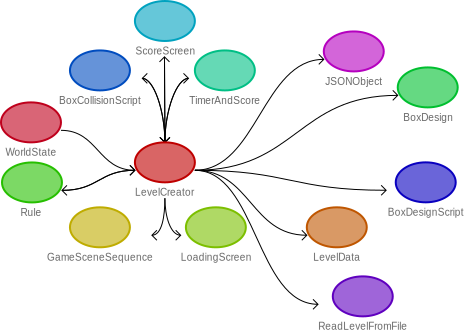
\includegraphics[width=0.7\textwidth]{images/LevelCreator_class_connectivity}
	\caption[LevelCreator class chart]{This is how we have connected classes to LevelCreator.}
	\label{fig:LevelCreator_chart}
\end{figure}

\todo{Represent parts of the class diagram to do point 3.3 in the 
product evaluation good.}

	\section{Program data}
		\label{sec:program_data}
		\todo{Write about the process we had for adding data. How Jakob 
implemented it at a late point when we were told that this was a 
"must do".}

	\newpage
	\section{Editor data}
		\label{sec:editor_data}
		\begin{wrapfigure}{l}{0.47\textwidth}
	\capstart
	\includegraphics[width=0.45\textwidth]{images/inspector.png}
	\caption{Default Unity inspector}
\end{wrapfigure}

To edit what the games does and how they look like we wanted meant that a lot of variables from our scripts had to be exposed.
By default Unity will expose all public variables in a script.
This includes scripts that the script want publicly available for other scripts to get or variables that should not be accessible for the
user but accessible for other scripts as the variable is only kept in the script but not used.

In our case we had a script that was to hold as much data about a minigame as possible.
This was so the game could be easily changed in the inspector of Unity without having to go into a script and manually edit.

The inspector quickly became crowded both by unnecessary variables that while they were needed they were not needed exposed all the time.
For instance there is no need to see the variables for creating a grid when you are creating a shape matching game.
And with the possibility of creating any of the minigames that we have implemented when you are creating a new game in a new scene in Unity 
this will lead to quite a lot of variables being exposed even if we try to share as many variables as possible.

To solve this problem we created a script to interact with the editor side of Unity to tell Unity how we
want the editor to look like instead of using the default behavior.
Doing it this way meant that we would have complete control over what is displayed and how.
Having complete control also means that we had to explicitly tell Unity what variables should go where, what name to show
for the field in the inspector, what values was acceptable and so on. 

Seen above are the data with the default inspector in Unity, what is not seen is the data about how cubes should look as this data 
is not in a format that Unity can show.
The other picture shows the inspector we built. 
Our inspector hides variables that is either not needed with the current settings or is not for the user to temper with.
This makes it easy to manipulate already made scenes / minigames in Unity or to swiftly create a new variant of a minigame.
And testing new configurations is quick and easy as all values and inputs are constricted to be only acceptable values.
This alleviates the user from a lot of responsibility and having to know about what goes on when data is changed as all of this is automated.

\begin{wrapfigure}{r}{0.47\textwidth}
	\capstart
	\vspace{-30pt}
	\includegraphics[width=0.45\textwidth]{images/inspector_edited.png}
	\caption{cogArc custom inspector}
	\label{fig:inspector_edited}
	\vspace{-15pt}
\end{wrapfigure}


	\newpage
	\section{Vuforia integration}
		\label{sec:AR_library_integration}
		% \subsection{Detached / Integrated AR library}
% \label{sect:input_handling}

\todo{Clean up this chapter! The section deviding is done harshly, so it definitely have to be fixed!}

When we started developing, none of us knew how Vuforia worked. Because of this
we had no specific plan for how we should handle the input. As we got into it,
we found that Vuforia gives us coordinates in space relative to the input
device / camera. From what we saw in the design document we wanted depth in the
games. We think this is logical since we try to combine the real 3D world with
our digital world presentation. Since we already got coordinates in space, we
thought that the input was convenient.

Nevertheless, the input did not fit our needs perfectly. In the "Total Sum"
game (\ref{game:total_sum}), we were building a tower to obtain the right
answer. I. e. "Combining Numbers" game (\ref{game:combining_numbers}) we were
putting cubes side by side in an horizontal fashion. We asked ourself how this
could be done when the camera could be all over the place.


\subsection{Different approaches}
One option could be to ask the player to have the camera only in one position
and then trust the user to obey our instructions. If trusting the user can be
avoided, we think we should. This relieves the user from potentially many
prerequisites. It also reduce the risk of complaint on the software when users
fail to follow the instructions and do not understand why the program doesn't
work as expected.

\paragraph{}

When we saw that the design document specified the creation of towers we came up with the idea to make use of the gyroscope that is found on many phones and tablets. The gyroscope allowed us to lock the input in to one or two axis for all the games. When the player was to build tower we could ignore horizontal connections and for all others we could ignore vertical connections. 

\paragraph{Frame-marker to cubes models}
Vuforia allows a small variety markers to give transforms(position, rotation and scale) to game-objects in unity. There is image-markers that can recognize an image even if it only sees a small part of the image. However the recommended max limit for image-markers was only five so at least for the cubes these were out of the question. There is also markers with shapes like cubes, cylinders, etc. but we had trouble getting these features to work, due to lack of documentation. And then there is the standard frame-marker which has to be completely visible to work but allows you to have up to 512 markers at once.\\
The standard way of using vuforia with unity is to set the gameObject to be a child of the marker in the game hierarchy. It will then be moved around, scale and rotate as the marker does and it will only be visible or active when the marker is recognized. This way does not allow the use more than one marker to find an object, markers cannot be children of each other. 

\begin{figure}[ht] 
        \capstart
        \centering  
        \includegraphics[width=\textwidth]{includes/simpleCubeMarkerModel.png}    
        \caption[Standard Cube-Marker model]{Simple visualization of the standard model.} 
        \label{fig:simple_cube_marker_model} 
\end{figure}

However you get very little control over it when you notice that the tracking is not quite as good as you want it to be. The cubes were jumpy, twitchy, disappear for a fraction of a frame and a few times even be consistently rotated more than 90 degrees off or remain on the screen long after the physical cube was taken away. The two last cases were quite rare and most of these could be blamed on the user not playing in optimal conditions or on the camera technology. But none the less it's a very volatile world to expose to algorithmic rules. We could not simply rely on the standard OnCollitionEnter, OnCollitionStay and  OnCollitionExit functions to handle the cubes connections. When a marker was lost, the virtual cube would disappear without calling OnCollitionExit(), leaving the program thinking the cubes were together when they may not have been. They were also so jumpy that they could make connections with cubes that weren't anywhere near them.\\
Our supervisor, Simon McCallum proposed the solution to separate the cubes and the markers to separate the volatile world from the game world. In the game world we could then freely manipulate it without changing the initial input. Also to make it easier to change the source of input so that we could quickly change the input to come from augmented reality glasses or from the web from someone else playing the game elsewhere instead of vuforia and the device camera.

\begin{figure}[ht] 
        \capstart
        \centering  
        \includegraphics[width=\textwidth]{includes/complexCubeMarkerModel.png}    
        \caption[Separated Cube-Marker model]{Simple visualization of the separated model.} 
        \label{fig:complex_cube_marker_model} 
\end{figure}

In this model the markers would pass their transforms to the cubes as function parameters. The cubes would then use these to position them selfs in the game world. This model was not the one we went with but it had many options we had to consider:
\begin{itemize}
  \item We could use a different marker to show where the table is and use this to position and rotate the cubes. The cubes can not be lower than the table and they have to lay flat if they are on the table. Considering the instability of frame-markers (we couldn't just use one) and the difficulty of getting the markers recognized (we couldn't use many), frame-marker were pretty much out of the picture. We could use an image-target as a tablecloth. We tried to set up image-targets, but we couldn't get the targets recognized. It could have been a problem with the paper or size, scale, resolution of the image, lighting conditions, setup and so on, but we decided to drop this.
  \item We could have used more than one marker for each cube, put one on each side and average their transforms. This could have helped make the cubes just a little more visible and stable, but it would create a lot of complexity. Using several markers increases the chance of one of them, particularly the ones that are the least visible to mess up the cubes position even if it's not as much due to the averaging. The complexity would be a lot extra work for us to create handling for all those optional markers and for the devices that have to run the program. Since we were developing for tablets and cellphones we tried not to push the limits to much. It wouldn't help all that much since the cubes are massive objects, and really just need one clearly visible marker to be placed perfectly in the game world.
  \item We could handle the activation and deactivation of the cubes our selfs. This we did actually attempt to do. The result was a lot more stable, pretty and even colorful than the standard Vuforia- / Unityway, but much worse in relation to game-play. The cubes would freeze in place on the screen, for short periods of time making it hard to see what was going on behind them and generally just feel very unnatural to play with. We could have done the same as Vuforia to hide them when the markers aren't visible, but then there wouldn't really be a point in doing it and we didn't manage to make manual version as natural. 
  \item We could show transparent cubes where the markers were, manipulate the transforms and then place the cubes there with no transparency. But this would just be an excuse, a way to make up for the unnatural way of handling the input and it would probably just distract the player from the game it self.
\end{itemize}


\subsection{Solution}
In the end we decided to use the standard way, with a way to easier set different parents than the frame-markers and use filtering on the game-world state before testing for goal completion, rather than modifying the cubes positions before displaying them to the user. We found this gave the cubes fairly natural and more relate-able and forgivable behavior and to be better for playing the game as players. This way shows the player the instable recognition of the markers, allowing him to adapt to it while keeping the world state that is being tested with the game rules to be a little more stable than it seems. Not by using individual manipulation, but by universal filtering to make the state stable.

	\section{Development changes and decisions}
		\label{sec:Developmentchangesanddecisions}
		Following is a list of decisions and changes we as a group made during the development of this project in chronological order.

\begin{enumerate}
	\item 09.jan: As many as possible mini games should be created in a dynamic way.
	\item 09.jan: Graphics for the system does not have to be more advanced than what is shown in the design document.
	\item 09.jan: The cubes need only to have basic collision between others to achieve the functionality we need for the games.
	\item 09.jan: Our focus should be on making as many games as possible within the framework and not on making  a few perfect ones.
	\item 24.jan: We decided to shift our focus to be more on the framework itself and not the games within the framework.
	\item 30.jan: Costas wants us to implement a variation of the mobile app Wooords to replace a few of the other mini games.
	\item 31.jan: We decide to look into the implementation of Wooords at a later date in the development as it is a interesting game and will enhance the finished app since it is not similar to the other mini games.
	\item 10.feb: The group, along with Costas have decided to drop the memory mini game and the path mini game described in the design document.
	\item 17.feb: In the design document it implies that the loading screens should have all time leader board and a high score for the player. This is not consistent with the rest of the design document nor with our planning document and it was decided to instead have a high score for the current player on the loading screen instead.
	\item 06.mar: The design of the boxes is set in the inspector during the making of the game in Unity, the design can therefore not be changed during runtime.
	\item 10.mar: We decided to look into detached / integrated use of a AR library.
	\item 18.mar: Pictures that will be used as textures on the cubes must be in a folder called "/Resources/BoxDesign/" to be able to properly load them since we are not able to extract the path of where a texture is stored on disc.
	\item 27.mar: The levels for mini games will be procedural generated unless you want to make a Wooords mini game, where the levels will be read from file since these levels can not be easily randomly generated.
	\item 29.apr: The restart button have been removed from the pause screen.
\end{enumerate}

\section{Framework instead of games}
In the beginning we wanted to make sure that we would be able to create all the games described in the design document, and after looking into how we should structure the programs and what scripts and the like could be shared between each of the mini games we realized that on the programming side of them there was little difference. We therefore decided upon focusing making a framework to work within instead of making each mini game special.

\section{Implementing a word game instead}
Shortly after beginning development and starting testing of the \gls{Frame Marker} we realized that the mini game \#5: Memory cubes as it was described in the design document was not implementable. Playing the game would make the player turn the cube upside down in the best case scenario or covering the frame marker and then turn the cube in the worst case. This caused us a lot of problems because of the way that Vuforia controls its frame markers. What Vuforia does when it is not tracking a frame marker or it loses the tracking is to deactivate the frame marker in the scene hierarchy which makes us unable to access any information contained within both the frame marker object itself and its children. This meant that we had no reliable way to detect if the player turned a cube to see the hidden mark under the cube or if it was simply re-detected by the tracker due either by the player obscuring the marker or something else obscuring the marker or the marker just being lost for a few frames. We brought this issue to our employer and after a short discussion we came to the conclusion to implement our own version of the mobile game Wooords and not make the mini game \#5: Memory cubes and also to not make mini game \#6: Path as the game was deemed % nu nu nu
Woords is a game where the player is presented with a jumble of words and a theme. The goal is to find as many or all the words in the level by combining the letters to make words.


\section{Dropping leader-board}
In the original design document we got there was mention of having the loading screen both instructions for the game and a global leader-board. Unity does not work well with net based activities 

\section{Putting textures in a special folder}
This decision is due to a limitation in Unity. When you place a object in the object field in the inspector it will give us a new instance of that object, in this case a texture. What it does not give us is where it is stored. This would not be a problem if Unity was able to serialize our data, but since we are storing our objects as a JSON object due to Unity not being able to serialize it we have to store it ourself and the name of the texture is the only data we can rely on. The name however does not include the path of where the object is stored, so when we are extracting the data back from JSON objects into textures we only have the name of the texture. So to avoid any confusion of duplicate names and avoiding searching for the texture we constrict the location of where it can be placed into a sub-folder in the Resources folder of Unity.

\section{Procedural generation over predetermined levels}
In the beginning of the development we were uncertain about whether we should create levels for the mini games with code or if it should be crafted by hand. We initially went for the possibility of both, however after discussing it with our employer we came to the conclusion that as many of the games as possible should have generated levels. The only mini game that is not suitable for random generation is mini game \#7: Wooord game, the Wooord game has a single file for each set up starting with the overall theme (example is: animal, this means that all the words are animal related), followed by a comma separated sequence of what words should be on the cubes and on the line under is a comma separated list of words that can be created with those words. To create more levels the file just have to continue with a new sequence of letters for the cubes to have and a new line of words that can be created.

\section{The restart button has been removed from the pause screen}
\todo{Jakob kan skrive om hvorfor den f\o{}rst \o dela alt, men at vi senere fikset den.}



\chapter{Product}
	\label{chap:product}

	\section{Visual}
		\label{sec:visual}
		% Visual

\begin{figure}[h]
	\centering
	\begin{minipage}{.5\textwidth}
		\capstart
		\centering
		\includegraphics[width=0.9\textwidth]{images/main_menu.png}
		\vspace{-10pt}
		\caption{Screenshot of the main menu.}
		\label{fig:main_menu}
	\end{minipage}%
	\begin{minipage}{.5\textwidth}
		\capstart
		\centering
		\includegraphics[width=0.9\textwidth]{images/loading_screen.png}
		\vspace{-10pt}
		\caption{Screenshot of a loading screen.}
		\label{fig:loading_screen}
	\end{minipage}%
\end{figure}

\paragraph{}
The main menu cosists of buttons that leads to each the minigames with each button having both the name of the corresponding
minigame and a small illulstration that gives the user a hint to what the user will do.
There is also the "YOUR NAME" and "EXIT" buttons. The "YOUR NAME" button will take the user to a new screen with a input field 
for chaning or setting their username whilst the "EXIT" button will exit the application.
The background behind the buttons is what the devices camera is currently seeing.

\paragraph{}
The second picture shows one of our loading screens, in this case it is the loading screen for \nameref{game:shape_match}.
The loading screens are comprised of two main elements and three smaller elements.
The main elements are the highscore list to the right and a description on the left.
These will introduce the user to what the goal for the minigame is and hopefully encourge the user to do their best everytime to improve the highscore.

The smaller elements are the titlebar that shows the name of the minigame followed by current level of the game and how many levels it has in total.
A button in the top left lets the user return to the main menu and lastly there's the "Start!" button that begins the game.

While in the menu the user can see what the camera is currently seeing in the background behind all these elements.

\begin{figure}[h]
	\centering
	\begin{minipage}{.5\textwidth}
		\capstart
		\centering
		\includegraphics[width=0.9\textwidth]{images/match_cubes.jpg}
		\vspace{-10pt}
		\caption{Screenshot of a mini-game.}
		\label{fig:screenshot_mini-game}
	\end{minipage}
\end{figure}

\begin{figure}[ht]
	\capstart
	\centering
	\includegraphics[width=0.8\textwidth]{images/MatchCubes}
	\caption{Match Cubes minigame}
	\label{fig:match_cubes}
\end{figure}

\paragraph{}
These two pcitures shows our current UI and what we had in the beginning.
Our first version used the default Unity style for both buttons and info boxes.
While it is funcitonal it is not very nice to look at and is too distracting in a enviroment such as this.
To rectify this we created our own UI styles to use instead of the default.
By removing as many distracting elements from the UI as possible we leave much more space open so the user can use more of the
screen to look for the cubes without having the UI be in the way.



\newpage
\section{Program flow chart}

\begin{figure}[ht]
	\capstart
	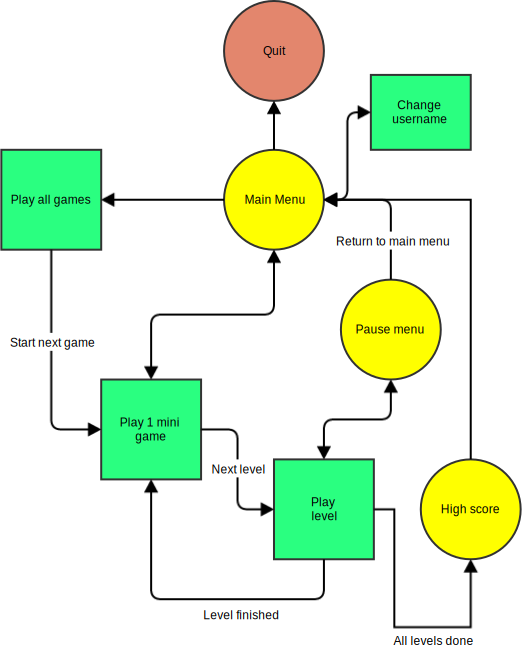
\includegraphics[width=\textwidth]{images/user_flow_chart}
	\caption[Program flow chart]{How a user maneuvers in the program.}
	\label{fig:program_flow_chart}
\end{figure}

Upon starting the program the user is presented with the main menu.
The main menu consists of four sets of buttons.

One set is the buttons that each lead to a single mini-game. 
When clicked they will take the player to the loading screen of the appropriate mini-game where the player can read instructions for the game and see current high-scores for that game.
After clicking the play button the user is taken into the game where the user can either play the mini-game or press the pause button.
If the user presses the pause button a pause screen is shown with the options of resuming the game, restarting from level one or go back to the main menu.

After the mini-game is completed the user is taken back to the loading screen if there is more levels left of the mini-game, otherwise the high-score list is shown.
The high-score lets the user go back to the main menu.

Back in the main menu, if the user presses the button "Change username" the user will be presented with a input field where a name can be entered, upon submitting a name the user will be brought back to the main menu.

If the user presses the "quit" button the application exits.

The last button on the main menu is the "Play all games" button. When the user presses this button it will play all the available mini-games in sequential order.

	\section{Adding new game}
		\label{sec:adding_new_game}
			\textbf{This is how you can make a game:}
	\begin{itemize}
		\item Open the startscene in Unity.
		\item In the scene hierarchy, click on "Main Menu" to open it in the
			inspector.
		\item Find the "Name Of Games" string array.
		\item Expand it by one and name your game in the new spot.
		\item Now create a new scene in Unity.
		\item Delete the everything in the hierachy for the new scene and add
			a prefab we have created called "New Game Creator Prefab".
		\item Now, in the inspector, click on the button "Add all needed to
			create a new game!".
		\item Now you can specify rules and get started.
		\item To run your game, go to "Build Settings" in Unity. Click on the
			button "Add Current" and then "Build And Run".
		\item And there you go!
	\end{itemize}

	\textbf{Extra:}
	\begin{itemize}
		\item To add an icon, create it and put it in the folder 
			"Assets/Resources/icons" with the same name you specified in "Main 
			Menu" (Startscene).
		\item You may want to adjust the variable "Buttons Per Row" in Main
			Menu to change the look of it.
	\end{itemize}


	\section{Application data}
		\label{sec:application_data}
		\todo{Which data are stored in the app and which data is sent to the
		network? This should be a summary of what we have written under
		development.}


	% \newpage
	\section{Usability}
		\label{sec:usability}
		\subsection{Skipping levels}
During a game there might come up situations where you just want to quit. At
first we did not have this possibility, but during the testing phase we figured
out that this was something that had to be included. Particularly during the
Pattern Memory game (\ref{game:pattern_memory}) we think this is necessary. In
that game you will need to remember a pattern. If you fail to do so, you may
spend much time trying and failing to get the right pattern and frustration can
raise to an unfortunate level. 

\subsection{Total Sum Hint}
In the Total Sum game (\ref{game:total_sum}) it can be quite frustrating to add up the numbers in your head before hand, especially if the number of cubes you have to add up is more than three. When the player puts together two or more cubes in the specified way, (standard is vertical, but in the Unity inspector the rule can be changed to the horizontal version, "human readable" ) a text will appear on the top box or last box in the line showing how much the current sum is. The hint will only appear on one tower / word.

\subsection{AR Implementation}
AR implantation is explained in more depth in \ref{subsec:framemarker_model}.
When we were implementing Vuforia we focused on usability rather than aesthetics. The twitching, incorrect rotation and disappearing of the cubes when using the standard way give the player more nuanced feedback about the conditions for the tracking and understanding for how it works. Even though we were having tracking problems it was better to not make changes. There were other ways that could make the cubes easier to get into and keep in view, which would make some games easier to do if playing in bad conditions. but also in another way make the game harder because cubes would get stuck on screen or be in wrong positions confusing the player.

\subsection{Light condition}
When playing a game the light conditions of the area being played in plays a big role in how easy it is for Vuforia to detect a marker.
If it is too dark there won't be enough light for Vuforia to discern the markers. 
Vuforia will still be able to find the markers but it might not find it as easy as expected.
We suspect this to be because of the contrast to the frame marker and the surroundings. 
If Vuforia can't detect the frame around the marker it won't register as a marker.
This is also noticeable when the lights are too bright.
When playing in a very bright room the paper the markers are printed on will start having specular highlights.
And with the specular highlights being almost white it is then the opposite of what Vuforia is searching for in a image.
We have found that unfortunately that the black portion of our boxes reflects the most light.
We have found that playing in a normally lit room or office are very ideal as the chance of it having 
very bright light sources or light sources being very close to the marker to be unlikely.
Offices or other work-rooms also tend to be well lit to avoid eyestrain.
\todo{Have someone competent read this.}

	\section{Feedback - reported problems}
		\label{sec:feedback}
		\begin{itemize}
	\item A friend from F\o{}rde tried the app on his Samsung S5. This caused his phone to restart. When he tried the app after it's restart, the phone only replied that the program had stopped.
	\item There has been reported that it was hard to install the program from
	our webpage. To do so, one need to accept programs from "unsafe" sources
	that are not on Google Play.
	\item People have asked for the app both for iOS and Windows Phone. We have
	tried to port cogARC to these platforms, but never succeeded. There may be
	some APIs and features that are not available in the Unity free edition.
	For Windows Phone the webcam is not available
	\cite{GettingStartedWindowsPhoneBuildUnity}, so that may be one of the
	problematic factors.
	\item Someone was observed to connect the frame markers by dragging
	on the screen from one of them to the other. This is probably since it is a
	new technology and may be most prominent the first time a person tries it.
	\item By trying on a smart phone someone was observed to hold it quite high
	in a sitting position. The reason was to see all the frame markers at the 
	same time. It was an uncomfortable position and the player started to 
	recognize it in their back. This was played without cubes, but with flat
	markers on the table. It may not be a problem when playing it as the
	employer have described -- with cubes in a sitting position with a tablet
	in front(bigger screen).
	\vspace{8pt}
	\item \nameref{game:pattern_memory}:
		\vspace{-8pt}
		\begin{itemize}
			\item Friend did not see the pattern in the corner when it
			started. A possible solution could be to put it at the middle of
			the screen to make it easier to see.
			\item Someone experienced that the game said the solution was both
			right and wrong at the same time. Algorithm optimization needed.
		\end{itemize}
	\item \hyperref[fig:pair_games]{Pair games}: Some got paired up without the user recognizing it. This
	we have seen before. A possible solution could be to show how many
	pairs that are left. On \nameref{game:shape_match}, it could e.g be 
	pictures of those that are left.
	\item \hyperref[subsec:vuforia]{Vuforia}: Marker recognition not good
	enough. Problem with seeing	markers are often problematic.
	\item General: Player felt frustrated and confused when not understanding
	the games. This changed upon completion of a level, where instead there 
	were rewarding feelings of joy and victory (\nameref{game:pattern_memory}).
\end{itemize}

	\section{Future Development}
		\label{sec:future_development}
		There are many ways to work further with the software we have started on.
The first thing we will propose is to do proper testing and fix the bugs that
will show up. Testing should uncover whether the functionality works as 
intended or not. It should also try to see if the games work as intended.

\begin{wrapfigure}{r}{0.6\textwidth}
	\capstart
	\centering
	\vspace{-10pt}
	\includegraphics[width=0.58\textwidth]{images/META1_website_image_resized}
	\vspace{-5pt}
	\caption[{META S}paceglasses - Early version]{{META} Spaceglasses. This
	depicts an early version that they sent during a chat conversation on 
	their webpage in January.}
	\vspace{-10pt}
	\label{fig:meta_spaceglasses}
\end{wrapfigure}

One other area that needs to be improved are the graphical user interface (GUI).
It will be a great id\'ea to get professional interaction designers to specify
and create the user interface. The current GUI are responsive to some extent, 
but it have proved not to be good enough. This is highly encouraged to get 
done.

\paragraph{}

When it comes to advancing the software, there are some points we would like 
to mention. One exciting thing to try is to port cogARC to wearable glasses.
Since the original plan was to implement the program for the \gls{Meta 
SpaceGlasses}, these will probably be good to try it on. From their webpage
\cite{MetaSpaceGlasses}, they now, at the 13th of May 2014, claims that new 
orders will start shipping in September. We will expect Kickstarter supporters 
to receive the product a bit before that, so it might be ready to test in only
a few months time if anyone would implement it.

Another advancement is to do something with the tracking and flickering of the 
markers. This is a disturbing factor in the games and would enhance the game
experience if it were fixed. One way is to use an other tracking library than
Vuforia, but there may be tricks that can be done locally to reduce the 
problem. One way can be to handle the input from the library in a more advanced
way.

\paragraph{}

From a more academic perspective, it would be good to look more into the actual
research value of cogARC. When looking at it from that angle, there may show up
several ways to enhance the software. Logging may change in what data that are
being logged and how the data is filtered, stored and used.

New games may be added to investigate in other cognitive functionalities than 
those that are already there. Some of the games that are implemented may be
filtered out, while others may change if they does not serve their purpose well.



\chapter{Summary}
	\label{chap:summary}

	\section{Goal acquisitions}
		\label{sec:goal_aquisitions}
		\begin{description}
	\item[Result goals]\ 
	\begin{itemize}
		\item 7 games.
		\item Adaptable framework.
		\item Viable bachelor thesis.
		\item Combine physical cubes and digital structures.
	\end{itemize}
\end{description}

These are the result goals we started out with. During the process some of them
were altered a little. Some of the game id\'eas were dropped due to technical
issues. Some were decided to be abandoned in conversation with our employer.
They were simply not interesting or necessary enough. This selection process
was done over time in the early phases of the project. In the end, we finished
every game that were planned. One of the games we dropped were implemented
close up to the deadline, but finalization with proper testing were not
prioritized. This shows that the framework is adaptable and it does not take
very long time to expand on it to create new simple game types.

The framework we made is flexible beyond what was required to make the
requested games.
The rules of games can easily be changed in Unity. 
There are several options for changing the difficulty of games, such as setting time limits, setting number of cubes used to form solutions and setting number of levels.
For the \nameref{game:wo0ord_game}, the file containing the tasks can easily be changed. 
The game description can be changed and the score system can to some degree be tweaked in the inspector.
Adding a new game in main menu may not be straight forward, but there is not
much to it. It is as described in \autoref{sec:adding_new_game}
\nameref{sec:adding_new_game}.


\todo{is this ok?}
In the scripts it is fairly easy to create long series of games. 
It is not added support for creating other series of several games or playing games in another order as this is coded into the behavior of the loading of scenes in the main menu.\\
We think we completed the task well and the \nameref{game:wo0ord_game} and the inspector-framework (\ref{sec:editor_data}) were big additions to the initial assignment. Time-wise we logged a little over 400 hours each, which is a little lower than expected, but not uncommon. So we believe we have made a viable bachelor thesis.\\
We turned the volatile environment seen by the cameras of the real world
into fairly stable arrays and lists and tested them against both preset 
and randomly created states. Some buggy behavior occurs, but most of this
is because the images from the camera are too bad for the trackers or because
of Vuforias tracking algorithms and therefore such that we have little or no control over the matter.\\

\begin{description}
	\item[Effect goals]\ 
	\begin{itemize}
		\item Support research.
		\item Experience with a game engine.
		\item Experience with a longer development process.
		\item Experience with digital space linked to reality.
	\end{itemize}
\end{description}
We cannot really say at this point how well our product will support the research, but our employer stated that he was pleased with the product and we were able to meet most of the requirements for logging events. 
So we reckon it will be at least a little useful.\\
We haven't had a lot experience with large projects and they have all been in different environments, coding languages and with different tools. 
So we had a lot of trouble in the beginning of the project figuring out how to structure, set up the scene hierarchy, where to put scripts and how to make scripts communicate.
As we implemented new features we went over the structure several times, improving it a little each time. 
The Unity project still shows signs of structural weaknesses we chose not to remove because it would mean a lot of refactoring-work. 
We believe that in future projects in Unity and similar we will be able to set much better structure because of the experience we gained in this project.\\
We didn't really explore the field of AR as much as our supervisor wanted us to, but we studied the possibilities. 
If the technology had been better we might have gone much deeper in this direction.


	\section{Group work evaluation}
		\label{sec:group_work}
		\todo{Evaluate the groupwork and have someone read this.}
As a group we worked very well together.
We worked together very closely throughout the entire development by sitting in a storage room in Mustad and we all became good friends and had very good synergy between us.
Disagreements were few and far between and none of them escalated to be more than heated discussions. Most of them were just miss-communication to begin with. 



	\section{Reflection}
		\label{sec:reflection}
			\todo{Read it and weep?}
In the end we got everything we wanted working.
We implemented all games mentioned in the design document as good as we possibly could except for the two games that we decided along with our employer to drop.
One of them was dropped due to limitations with the technology we are using and the other one was dropped as our employer found it to be unnecessary if we implemented the \nameref{game:wo0ord_game}.

Although we tested everything during development we would still like to have more time to test on more devices and have more playtesters.
We would also like to completely redo everything we coded.
Some parts of the code stills shows that we had little experience with Unity and our code hierarchy definitely could do with a overhaul.
But even with this we have a product that can be easily added on to create code to support more games later or to change the games already coded.

In the end we have a project that we are pleased with, where we learned a lot about a new programs, a new coding language and how it is to work on a big project.

		
	\section{Conclution}
		\label{sec:conclution}
		This project have been the largest project we have worked on so far, so we have learned
a lot. We have got first hand experience about the synergy between planning and development.
Even though we planned as best as we could in the beginning of the project we now see that we could have approached the planning differently. One option could be to plan a structure ahead and hope that we could apply it in an unknown environment. Another option could be to start learning Unity from the very beginning to learn its inner workings, and then start planning.
We have seen that getting people to test and giving feedback on the product is very helpful and that it often gives insight we could not foresee. That led us to think that more feedback and testing would make the end product better.

The codebase we have now show both that we had no experience in the beginning and that we now know our tools very well. If we would have done it again there is one big change we would have done. That is to change from UnityScript to C\#. UnityScript was part of the task description, but we agree as a group that the development process would probably have been easier with C\#. Our understanding is that Unity’s implementation of JavaScript is a much less mature language, therefore one would be better off by using C\#. If anyone plan to build extensively upon our work, our advice is to use our codebase as inspiration and port cogArc from Unity’s JavaScript.

When we look back at the process we have had during this graduation project, there are several things we would like to point out.
In our view the school has not been good enough in taking care of its students. Limited work space for development are not good for cooperation and group projects. We have also felt that the way information is shared has not been structured enough. During the two first months our supervisor was hard to get a hold of and our planning phase were affected by this.

We have tried to do the best out the situation by making some space in a storage room and used it as our office. We sent a mail to the administration about the information that was presented on Fronter and proposed several ideas for making it more lucid. Much were improved during the following days. When we needed extra guidance, we have asked for other opinions from other people, including our employer.

In the end we think the bachelor project has given us valuable experiences that will be very useful for us. We have seen much of what we can do better, but we have also seen that we are actually capable of building software from a design document.


\vfill{}

\begin{center}
	In preparing for battle\\
	I have always found that plans are useless,\\
	but planning is indispensable. \\
	\paragraph{}
	\hfill{}\hfill{} Dwight D. Eisenhower \cite{Eisenhower}\hfill{}\hfill{}
\end{center}

\vfill{}

% Glossary list
\printnoidxglossary[sort=word]

% References
\bibliographystyle{classes/gucthesis}
\bibliography{includes/cogARC_bibliography}


%%%%%%%%%%%%%%%%%%%%%%%%%%%%%%%%%%%%%%%%%%%%%%%%%%%%%%%%%%%%%%%%%%%%%%%%%%%%%%%
%%% APPENDICES STARTS HERE %%%%%%%%%%%%%%%%%%%%%%%%%%%%%%%%%%%%%%%%%%%%%%%%%%%%
%%%%%%%%%%%%%%%%%%%%%%%%%%%%%%%%%%%%%%%%%%%%%%%%%%%%%%%%%%%%%%%%%%%%%%%%%%%%%%%

% Hack to get appendices on a new page in table of content
\addtocontents{toc}{~}
\addtocontents{toc}{\\}
\addtocontents{toc}{\\}

% Hack to stop summary page count here
\label{STOP_SUMMARY_PAGECOUNT}

\clearpage
\appendix %after this line all chapters will have letters instead of numbers
\addappheadtotoc
\appendixpage

% Let included pdf's get page numbering
\includepdfset{pagecommand=\thispagestyle{plain}}

%%%%%%%%%%%%%%%%%%%%%%%%%%%%%%%%%%%%%%%%%%%%%%%%%%%%%%%%%%%%%%%%%%%%%%%%%%%%%%%
%%% PROJECT DESCRIPTION %%%%%%%%%%%%%%%%%%%%%%%%%%%%%%%%%%%%%%%%%%%%%%%%%%%%%%%
% Project description
\clearpage
\phantomsection
\addtocounter{chapter}{1}
\addcontentsline{toc}{chapter}{\Alph{chapter} Project description}
\includepdf{external_docs/AR_project}

%%%%%%%%%%%%%%%%%%%%%%%%%%%%%%%%%%%%%%%%%%%%%%%%%%%%%%%%%%%%%%%%%%%%%%%%%%%%%%%
%%% EMPLOYERS DESIGN DOCUMENT %%%%%%%%%%%%%%%%%%%%%%%%%%%%%%%%%%%%%%%%%%%%%%%%%
\clearpage
\phantomsection
\addtocounter{chapter}{1}
\addcontentsline{toc}{chapter}{\Alph{chapter} Employer's design document}
\includepdf[pages=-]{external_docs/DESIGN_DOCUMENT_v2}

%%%%%%%%%%%%%%%%%%%%%%%%%%%%%%%%%%%%%%%%%%%%%%%%%%%%%%%%%%%%%%%%%%%%%%%%%%%%%%%
%%% PROJECT PREPLAN %%%%%%%%%%%%%%%%%%%%%%%%%%%%%%%%%%%%%%%%%%%%%%%%%%%%%%%%%%%
\clearpage
\phantomsection
\addtocounter{chapter}{1}
\addcontentsline{toc}{chapter}{\Alph{chapter} Project pre-plan}
\includepdf[pages=-]{external_docs/Project_plan}

%%%%%%%%%%%%%%%%%%%%%%%%%%%%%%%%%%%%%%%%%%%%%%%%%%%%%%%%%%%%%%%%%%%%%%%%%%%%%%%
%%% PROJECT PREPLAN %%%%%%%%%%%%%%%%%%%%%%%%%%%%%%%%%%%%%%%%%%%%%%%%%%%%%%%%%%%
\clearpage
\phantomsection
\addtocounter{chapter}{1}
\addcontentsline{toc}{chapter}{\Alph{chapter} Project agreement}
\includepdf[pages=-]{external_docs/Project_agreement}

%%%%%%%%%%%%%%%%%%%%%%%%%%%%%%%%%%%%%%%%%%%%%%%%%%%%%%%%%%%%%%%%%%%%%%%%%%%%%%%
%%% TIME MANAGEMENT %%%%%%%%%%%%%%%%%%%%%%%%%%%%%%%%%%%%%%%%%%%%%%%%%%%%%%%%%%%
\clearpage
\phantomsection
\label{appx:time_management}

\addtocounter{chapter}{1}
\addcontentsline{toc}{chapter}{\Alph{chapter} Time management}

\addtocounter{section}{1}
\addcontentsline{toc}{section}{Summary report}
\includepdf[pages=1]{external_docs/summary-report_toggl}

\phantomsection
\addtocounter{section}{1}
\addcontentsline{toc}{section}{Detailed report}
\includepdf[pages=-]{external_docs/detailed-report_toggl}

%%%%%%%%%%%%%%%%%%%%%%%%%%%%%%%%%%%%%%%%%%%%%%%%%%%%%%%%%%%%%%%%%%%%%%%%%%%%%%%
%%% GIT COMMITLOG %%%%%%%%%%%%%%%%%%%%%%%%%%%%%%%%%%%%%%%%%%%%%%%%%%%%%%%%%%%%%
\clearpage
\phantomsection
\addtocounter{chapter}{1}
\addcontentsline{toc}{chapter}{\Alph{chapter} GIT commitlog}
\includepdf[pages=-]{external_docs/git_log_unityproject}

\end{document}